\documentclass[aspectratio=43, t]{beamer}
\usetheme{CSCS}

\usepackage{amsmath}
\usepackage{amssymb}
\usepackage{fontspec}
\usepackage{unicode-math}
\usepackage{pgfpages}
\usepackage{minted}
\usepackage{xurl}
\usepackage{hyperref}
\usepackage{booktabs}
\usepackage{multicol}
\usepackage{physics}
\usepackage{pgfplots}
\usepackage{tikzpagenodes}
\usetikzlibrary{arrows.meta}

\renewcommand{\laplacian}{\increment}

\setminted{autogobble, obeytabs, tabsize=2, breaklines = true}
\setsansfont[Scale = 0.85]{TeX Gyre Heros}
\pgfplotsset{
	height = 8cm,
	compat = newest,
	results/.style = {
		xbar,
		xmin = 0,
		xmax = 20,
		ytick = data,
		nodes near coords,
		nodes near coords align = horizontal,
		every axis plot post/.append style = {
			cscsred,
		},
		xticklabel style = {
			/pgf/number format/assume math mode = true,
			font = \sffamily,
		},
		yticklabel style = {
			font = \footnotesize,
			align = right,
			text width = 3cm,
			execute at begin node = \setlength{\baselineskip}{7pt},
		},
		node near coords style = {
			/pgf/number format/assume math mode = true,
			font = \sffamily,
		},
	},
}

% define footer text
\newcommand{\footlinetext}{Rust Webinar}

% Select the image for the title page
%\newcommand{\picturetitle}{cscs_images/image3.pdf}
\newcommand{\picturetitle}{cscs_images/image5.pdf}
%\newcommand{\picturetitle}{cscs_images/image6.pdf}

\author{Michal Sudwoj}
\title{Rust programming language in high-performance computing}
\subtitle{Final Presentation}
\date{25.08.2020}

\setbeameroption{show notes on second screen = right}
\begin{document}
% disable Pygment error highlighting
\renewcommand{\fcolorbox}[4][]{#4}

\begin{frame}[plain, c]
	\titlepage
\end{frame}

\section*{Introduction}
\begin{frame}
	\frametitle{\secname}
	\begin{itemize}
		\item Fortran, C++ established languages for HPC
		\item Rust offers safety (borrow checker)
		\item Does it have (the features) that it needs?
			\begin{itemize}
				\item see \emph{Introduction to Rust} presentation
			\end{itemize}
		\item \textbf{Is it fast enough?}
	\end{itemize}
\end{frame}

\begin{frame}
	\frametitle{Problem}
	\begin{itemize}
		\item fourth-order numerical diffusion in $xy$-plane
			\[ \pdv{\phi}{t} = -\alpha_{4} \nabla^{4}_{xy} \phi = \underbrace{-\alpha_{4} \laplacian^{2}_{xy} \phi}_{\texttt{inline}} = \underbrace{-\alpha_{4} \laplacian_{xy} (\laplacian_{xy} \phi)}_{\texttt{laplap}} \]
		\item on unit cube
		\item boundary conditions: \( \partial_{\Omega} = 0 \)
	\end{itemize}
\end{frame}

\begin{frame}
	\frametitle{Initial conditions}
	\centering
	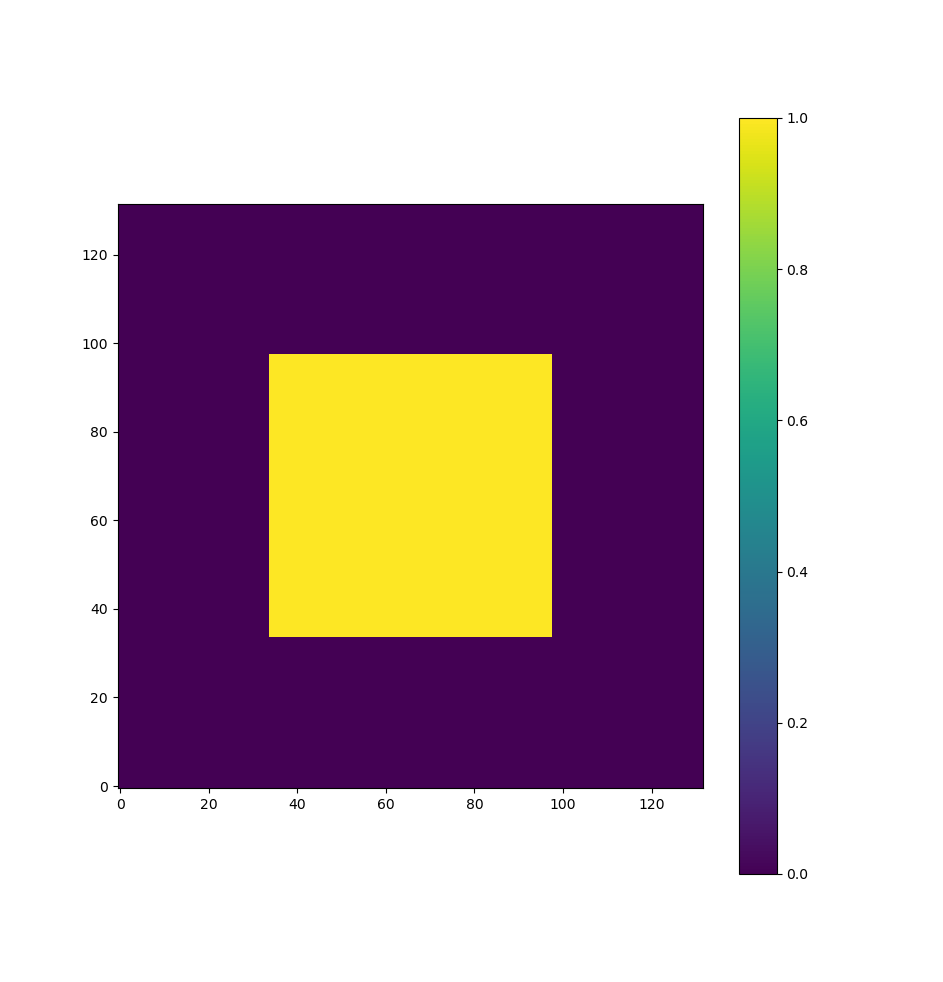
\includegraphics[width = \textwidth, height = \textheight, keepaspectratio]{in_field}
	\par
\end{frame}

\begin{frame}
	\frametitle{Result}
	\centering
	\includegraphics[width = \textwidth, height = \textheight, keepaspectratio]{out_field}
	\par
\end{frame}

\begin{frame}
	\frametitle{Benchmark}
	\begin{itemize}
		\item Fortran, C++, Rust
		\item Algorithms: \texttt{laplap}, \texttt{inline}
		\item Toolchains
			\begin{itemize}
				\item Fortran, C++: GNU, Cray, Intel, PGI
				\item Rust: \texttt{rustc}
			\end{itemize}
		\item Sequential
		\item Parallel
			\begin{itemize}
				\item Fortran, C++: OpenMP
				\item Rust: Rayon
			\end{itemize}
		\item GPU
			\begin{itemize}
				\item Fortran, C++: OpenACC, OpenMP offloading, CUDA
				\item Rust: Accel
			\end{itemize}
	\end{itemize}
	\note[item]{MPI works, but not enough time to debug the partitioner}

	$\implies$ 52 versions $\times$ 4 grid sizes
\end{frame}

\begin{frame}[fragile]
	\begin{itemize}
		\item arrays in column-major order
		\item \texttt{-O3} or equivalent
		\item no LTO
		\item optimization reports
		\item shared libraries
		\item C interface \\
			\begin{minted}{C}
				void diffuse(
					float * in_field,
					float * out_field,
					size_t  nx,
					size_t  ny,
					size_t  nz,
					size_t  num_halo,
					float   alpha,
					size_t  num_iter
				)
			\end{minted}
	\end{itemize}

	\note[item]{Show code on gitlab}
\end{frame}

\section*{Results}
\begin{frame}
	\centering
	\includegraphics[width = \textwidth, height = \textheight, keepaspectratio]{weak_scaling_seq}
	\par
\end{frame}

\begin{frame}
	\centering
	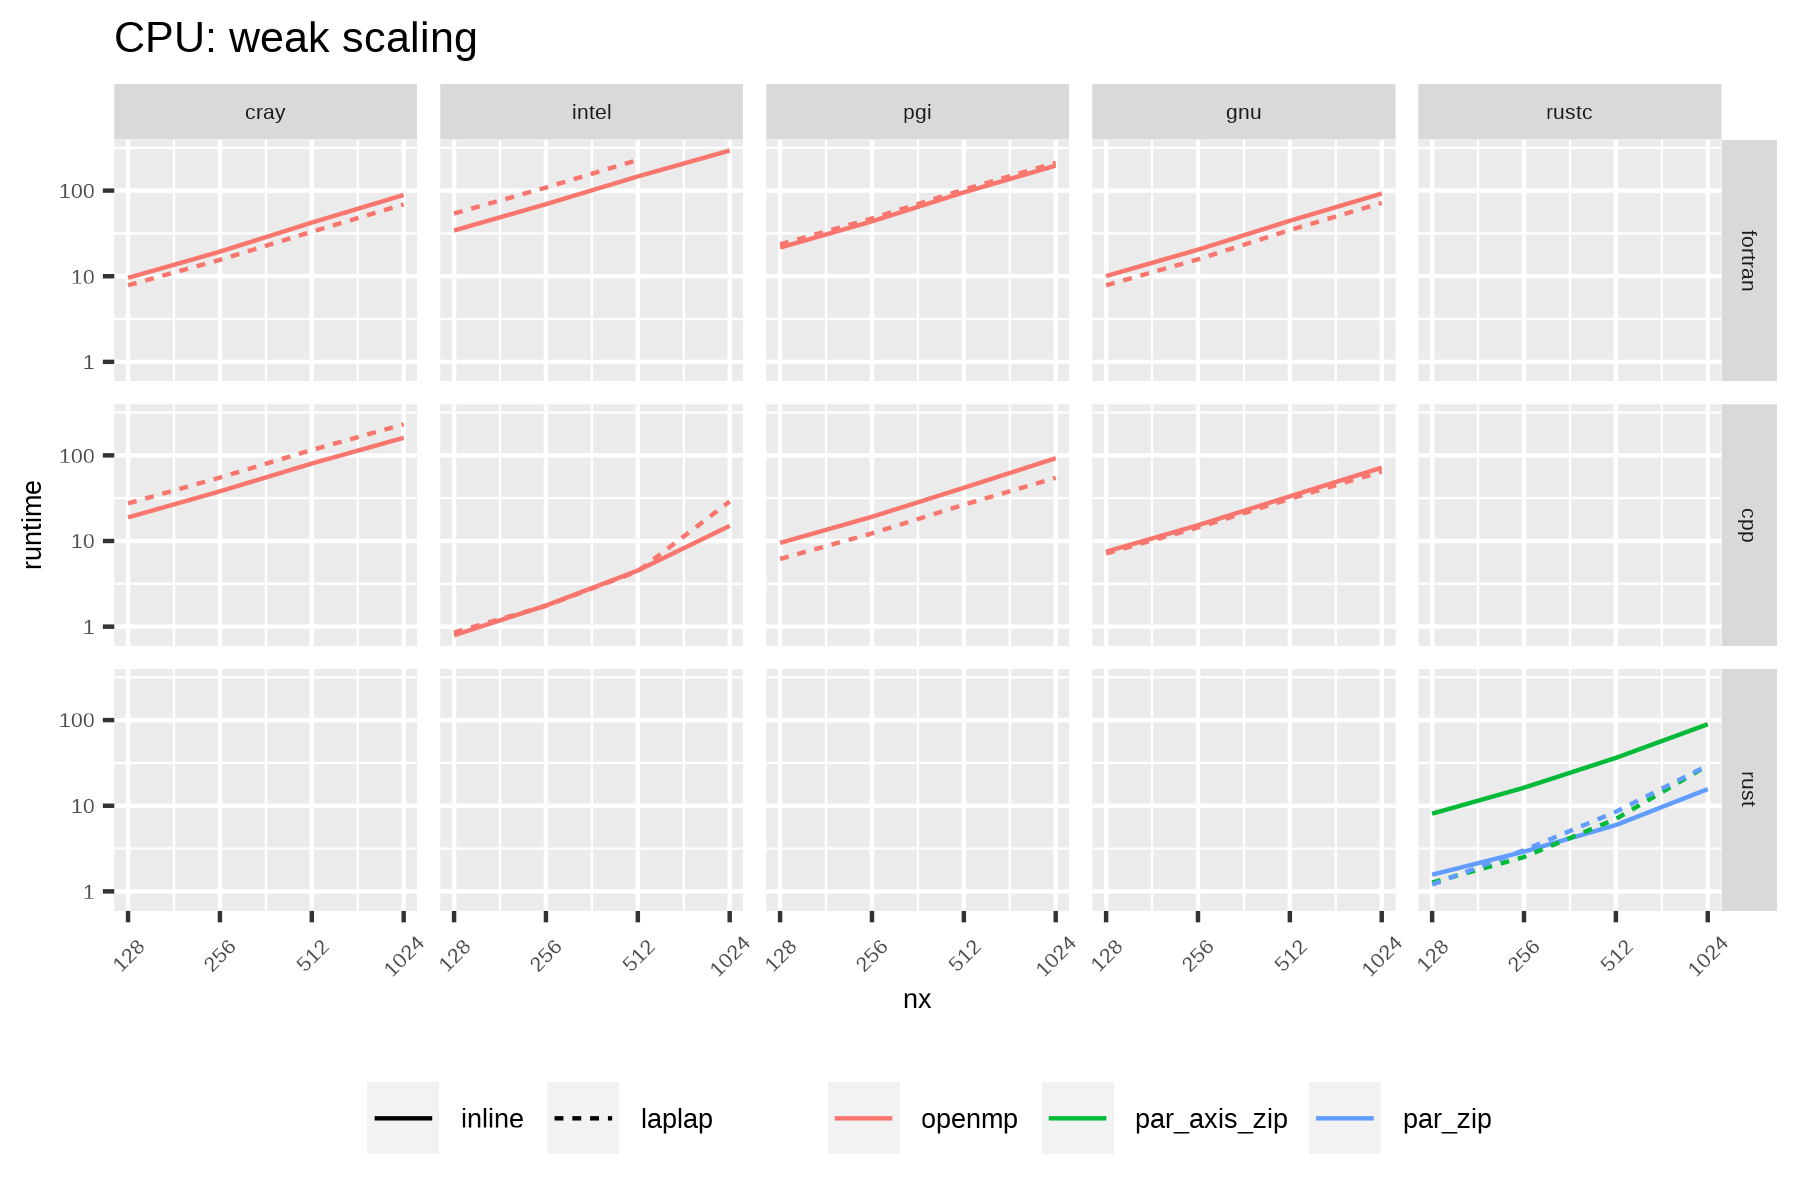
\includegraphics[width = \textwidth, height = \textheight, keepaspectratio]{weak_scaling_cpu}
	\par
\end{frame}

\begin{frame}
	\centering
	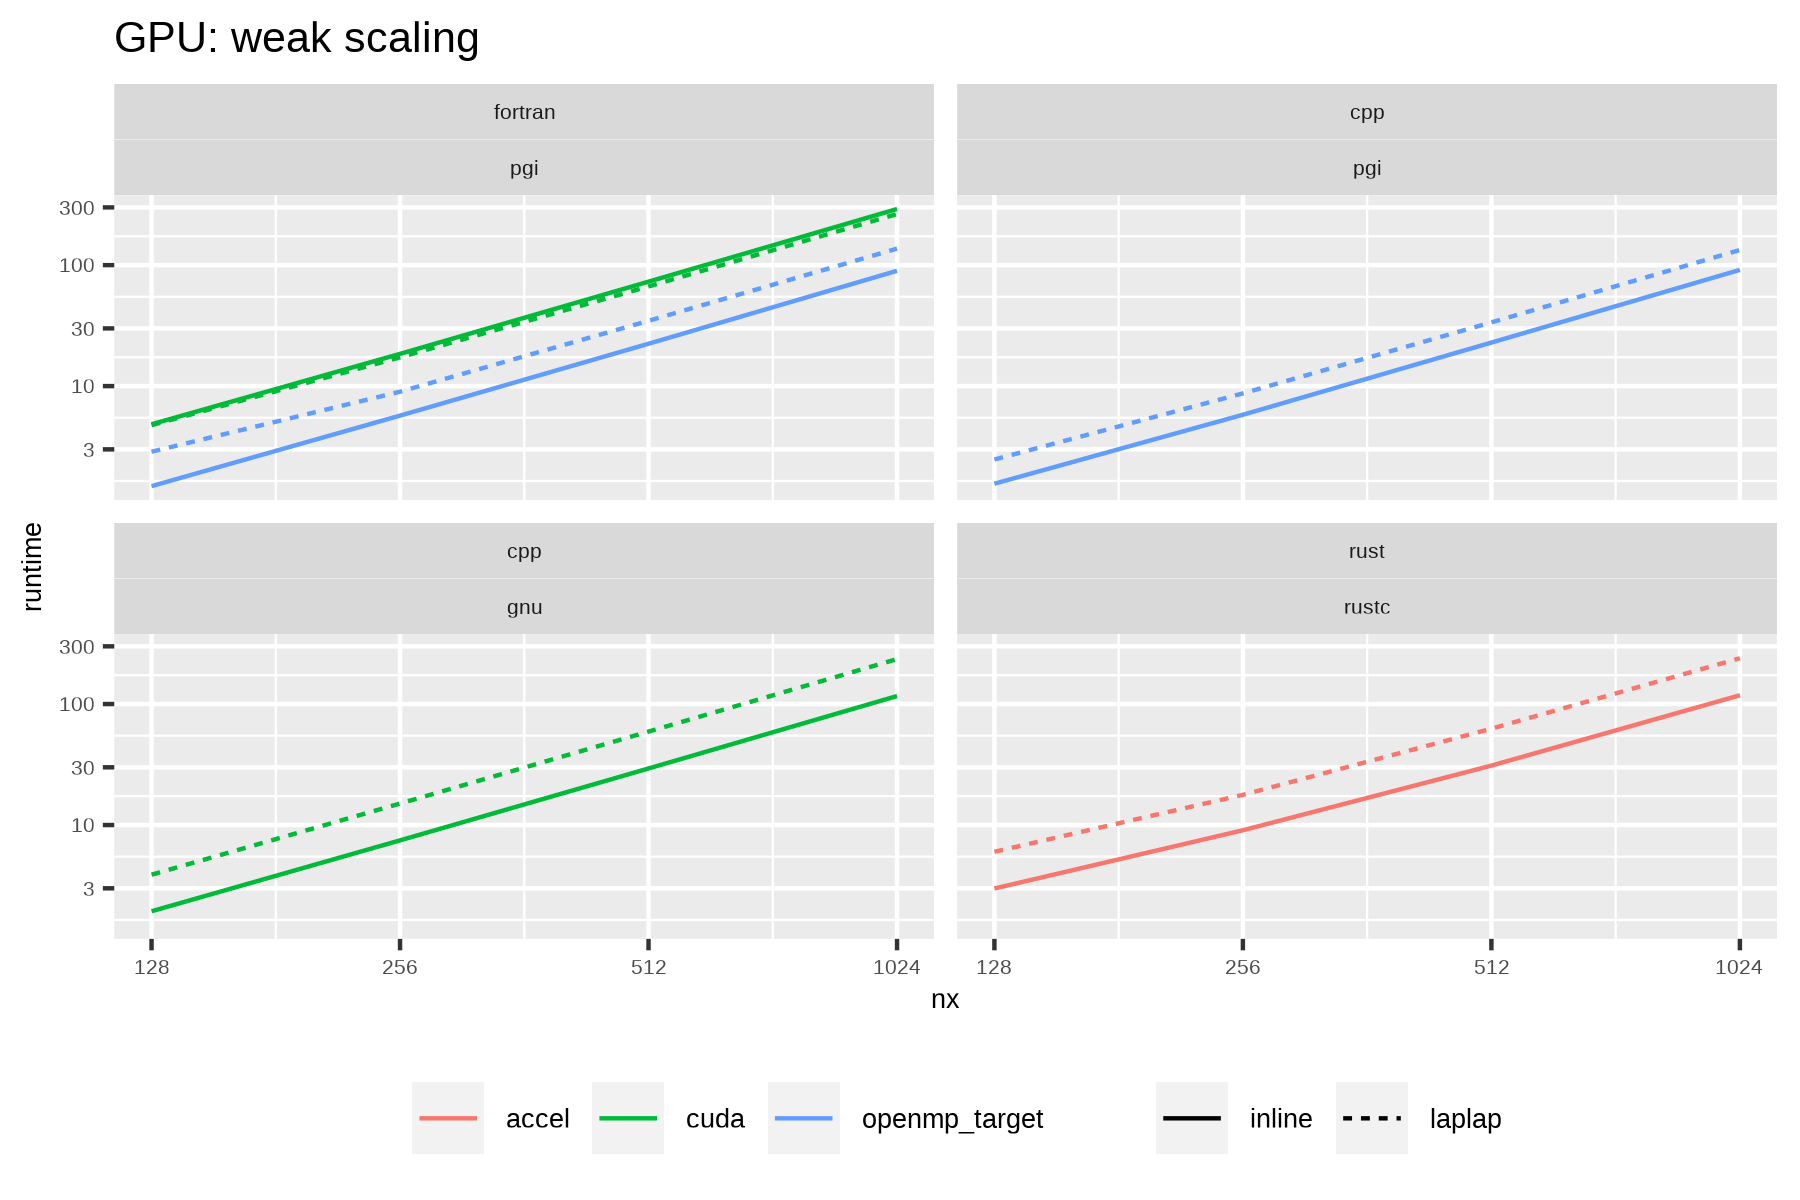
\includegraphics[width = \textwidth, height = \textheight, keepaspectratio]{weak_scaling_gpu}
	\par
\end{frame}

\section*{Conclusions}
\begin{frame}
	\frametitle{\secname}
	\begin{itemize}
		\item[$+$] Rust fast enough for scientific software
		\item[$+$]    Safer code
		\item[$+$]    Clearer error messages
		\item[$-$]    Support for certain features is lacking
		\item[$\sim$] All languages sometimes lead to lots of boilerplate
	\end{itemize}

	\note[item]{Rust compiler does good job of vectorizing code}
	\note[item]{Rust: clear what you get}
	\note[item]{Fortran/C++: different support, many bugs}
	\note[item]{GNU doesn't warn about lack of offloading}
	\note[item]{Cray sometimes silently generates invalid PTX code}
\end{frame}

\subsection*{Reccomendations}
\begin{frame}
	\frametitle{\subsecname}
	\begin{itemize}
		\item Today
			\begin{itemize}
				\item Rust for frontend/driver
			\end{itemize}
		\item Tomorrow (some effort required)
			\begin{itemize}
				\item GPU support
				\item Evolve \texttt{ndarray}
				\item ScaLAPACK bindings, \textellipsis
			\end{itemize}
		\item $\implies$ continue to pursue Rust in HPC
			\begin{itemize}
				\item it has potential
			\end{itemize}
	\end{itemize}

	See:
	\begin{itemize}
		\item \url{https://www.arewelearningyet.com/scientific-computing/}
		\item \url{https://www.arewelearningyet.com/gpu-computing/}
		\item \url{https://git.cscs.ch/msudwoj/rust-in-hpc}
	\end{itemize}

	\note[item]{With Cray and Intel moving to LLVM, cross-language LTO soon?}
\end{frame}

\begin{frame}[fragile]
	\frametitle{Start using Rust today!}
	\begin{minted}{console}
		> curl https://sh.rustup.rs -sSf | sh
		> rustup toolchain install nightly
		> rustup target add nvptx64-nvidia-cuda
		> # On Piz Daint
		> export
		>   CARGO_TARGET_X86_64_UNKNOWN_LINUX_GNU_RUSTFLAGS="
		>     -C target-cpu=haswell
		>     -C relocation-model=dynamic-no-pic
		>   "
		>   CARGO_TARGET_NVPTX64_NVIDIA_CUDA_RUSTFLAGS="
		>     -C target-cpu=sm_60
		>     -C target-feature=+sm_60,+ptx60
		>     -C relocation-model=dynamic-no-pic
		>   "
		>   MPICC=cc
		> cargo install ptx-linker
		\end{minted}
\end{frame}

\end{document}
